
\documentclass[12pt,  a4paper, twoside]{article} 
\usepackage[utf8]{inputenc} %For å kunne bruke æøå uten spesialkommandoer
\usepackage[norsk]{babel}   %For å få norske navn på figurer, tabeller, bibliografi
\usepackage{graphicx}  %For å inkludere figurer
\usepackage{amsfonts}  
\usepackage{amsmath}
\usepackage{fullpage}
\usepackage{caption}
\usepackage{import}
\usepackage{tabu}
\usepackage{longtable}
\usepackage[version=3]{mhchem}
\captionsetup{width=0.80\textwidth}
\captionsetup{font=small}
\usepackage{booktabs}
\usepackage{listings}
\usepackage[superscript]{cite}
\usepackage{hyperref}           % For inkludering av linker
\usepackage{siunitx}
\usepackage{pdfpages} % For å inkludere pdf-vedlegg!
\usepackage{cleveref}
\usepackage{parskip}
\graphicspath{ {Bilder/} }
\usepackage{float}


\title{CO_2-fangst \\ TKP4120 - Gruppe 25}
\author{Joachim Ågotnes \\Bård Bergerud\\Eirik Nygård\\Martin-Kristofer Helgeland-Rossavik}
\date{}


\begin{document}
\pagenumbering{gobble}
\maketitle
\begin{figure}[h]  
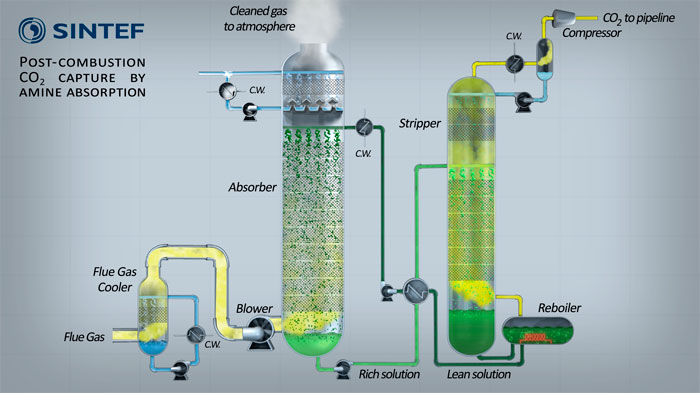
\includegraphics[scale=0.5]{Forsidebilde.jpg}
\centering
\end{figure}


\cleardoublepage

\section*{Sammendrag}
\import{sections/}{Sammendrag.tex}

\newpage
\tableofcontents
\newpage

\pagenumbering{arabic}

\section{Innledning}
\import{sections/}{Innledning.tex}

\section{Prosessbeskrivelse}
\import{sections/}{Prosessbeskrivelse.tex}

\section{Metode}
\import{sections/}{Metode.tex}

\section{Resultater og diskusjon}
\import{sections/}{Resultater_og_diskusjon.tex}

\section{Konklusjon}
\import{sections/}{Konklusjon.tex}

\import{sections/}{Referanser.tex}



\end{document}

